\chapter{Využitie knižnice Snap.svg}
Táto kapitola je o spôsoboch realizácie vizualizácie grafických komponentov cez JavaScriptovú knižnicu Snap.svg. 

\section{Porovnanie Snap.svg API a SVG SMIL}
Animovanie vektorov je jednoduchšie cez knižnicu Snap.svg ako cez SVG SMIL.  V nasledujúcom príklade je vykreslený a animovaný obdĺžnik cez SVG SMIL. Animácia spočíva v zmene šírky obdĺžnika z 50 na 100 pixlov.
\begin{lstlisting}[language = html]
<svg>
	<rect x="10" y="10" width="50" height="30">
		<animate attributeName="width"  to="100" fill="freeze"  
		dur="10s"</rect>
</svg>
\end{lstlisting}

Nakreslí sa obdĺžnik na súradniciach (10, 10) s šírkou 50, a výškou 30 použitím elementu $<$rect$>$. Zoskupený element $<$animate$>$ definuje animáciu zmeny šírky obdĺžnika na šírku 100 px, ktorá trvá desať sekúnd. Kde fill="freeze" je použité na zachovanie stavu obdĺžnika po ukončení animácie. Inak by bola nastavená znova na 50 px. \cite[p.~9]{Dawber}

Ekvivalent k animácii cez Snap.svg API v nasledujúcom príklade:

\begin{lstlisting}
paper = Snap();
var rect = paper.rect(10, 10, 50, 30);
rect.animate({
width: 100
}, 10000);
\end{lstlisting}

Syntax metód animate a rect je výstižnejšia a lepšia na pochopenie. Snap sa tiež dobre integruje s inými knižnicami. V práci som využívala iba Snap.svg knižnicu.  


\section{Inicializácia plátna na kreslenie - Snap()}
Na to, aby sme boli schopní kresliť grafické komponenty, tak potrebujeme definovať miesto, kde budú vykreslené. Viditeľná oblasť okna prehliadača alebo viewport, definuje oblasť, v ktorej sa vykreslí komponent na plátno. SVG špecifikácia referuje ako miesto vykreslenia seba ako viewport. 
Inak povedané viewport je akákoľvek obdĺžniková oblasť. Okno prehliadača je referencia na viewport a kresliaca oblasť je plátno.   \cite{Dawber}


\subsection{Súradnice plátna}
Vytvorenie plátna cez Snap konštruktor sa dá urobiť viacerými spôsobmi. Preto je potrebné vedieť súradnice plátna.  

Na to, aby bolo plátno zobraziteľné vo webovom prehliadači na rôznych zariadeniach musia byť nastavené nasledujúce atribúty: 
 \begin{itemize}
 	\item definovaný viewBox,
 	\item výška a šírka plátna musí byť v relatívnych rozmeroch, najlepšie nastavená na 100\%
 \end{itemize}

Nasledujúci príkaz zadefinuje plátno s rozmermi šírka je 300 a výška 200. 
\begin{lstlisting}
var paper = Snap(300, 200);
\end{lstlisting}

Na obrázku \ref{fig:suradnice1}  je znázornená východzí súradnicový systém plátna vytvoreného cez Snap konštruktor. 
Začiatok súradníc na osi x, y je rovné nule. Bod na plátne so súradnicami x = 300, y = 200 alebo (300, 200) vo vektorovom zápisu je bod 300px vpravo od začiatku x-ovej osi a 200px dole od počiatku y-ovej osi. 

\begin{center}
	\begin{figure}[H]
		\centering
		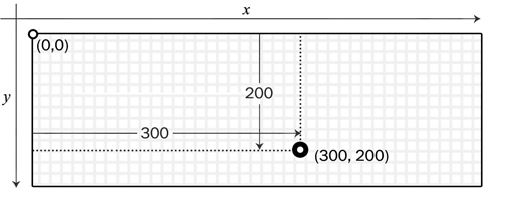
\includegraphics[width=0.5\linewidth]{obrazky/suradnice1}
		\caption{Súradnicový systém plátna s bodom (300, 200) v Snap.svg knižnici}
		\label{fig:suradnice1}
	\end{figure}
\end{center}

\subsection{DOM element}
Sú situácie, kde je potrebné použiť existujúci DOM element ako kontajner pre plátno než viewport. Ako element môžeme použiť napríklad:
\begin{lstlisting}
<div id="mojePlatno"></div>  
\end{lstlisting}

Nasledujúcim kódom vytvorím 500px široké a 300px vysoké plátno.

\begin{lstlisting}
var paper = Snap("mojePlatno", 500, 300);
\end{lstlisting}

Keď využívam túto formu konštruktora, tak prvý parameter v metóde je ID elementu. V prípade, že nie je udaný vykreslí sa na najbližšie voľné miesto. Alternatívne sa dá prvý parameter DOM element napísať nasledovným spôsobom: 
\begin{lstlisting}
Snap(document.getElementById('mojePlatno'), 500, 300);
\end{lstlisting}



\subsubsection{\acs*{SVG} v HTML dokumente}

Grafický komponent vo formáte .svg môže byť zobrazený buď ako inline v HTML dokumente, alebo ako vloženým samostatného .svg súboru. 
V tabuľke \ref{vytvorenie:SVG} sú vymenované HTML tagy na zobrazenie SVG. 


\begin{table}[H]
	\begin{center}
		\begin{tabular}{|l|l|}
			\hline \textbf{Technika (tag)} & \textbf{Popis} \\ 
		
			\hline $<$embed$>$ & Načíta vytvorený SVG súbor.  \\ 
			\hline $<$object$>$ & Vytvorí objekt SVG  \\ 
			\hline $<$iframe$>$ & Zobrazí SVG v rámci  \\ 
            \hline $<$img$>$ & Zobrazí obrázok s SVG obsahom   \\
			\hline Inline $<$svg$>$ & Vytvorí SVG   \\ 
             
			\hline 
		\end{tabular} 
	\end{center}
	\caption{Spôsoby zobrazenia SVG elementu v HTML dokumente}
	\label{vytvorenie:SVG}
\end{table}


Príklady načítania SVG v HTML dokumente pre tag Image:
\begin{lstlisting}
<img src="stanica2.svg" width = "50" height= "50" />
\end{lstlisting}


\section{Kreslenie základných tvarov cez knižnicu Snap.svg}

Snap.svg API poskytuje metódy na kreslenie jednoduchých tvarov. V tabuľke~\ref{porovnanieSVG:Snap} sú základné tvary, ich ekvivalentné vyjadrenie v SVG ako elementy, a  príkazy na vytvorenie nových elementov cez Snap.svg. Keďže sa jedná o vektorovú grafiku, tak pre elementy vytvorené cez SVG alebo Snap.svg platia rovnaké atribúty. Líši sa iba spôsob zápisu. 

\begin{table}[H]
	\begin{center}
		\begin{tabular}{|l|l|l|l|}
			\hline \textbf{Tvar} & \textbf{SVG element} & \textbf{Snap.svg API} & \textbf{Atribúty} \\  \hline
			\hline Obdlžnik & $<$rect$>$ & .rect() & x, y, šírka, výška, rx, ry \\ 
			\hline Kruh & $<$circle$>$ & .circle() & r, x, y, cx, cy, rx, ry \\ 
			\hline Elipsa & $<$ellipse $>$ & .ellipse() & x, y, cx, cy, rx, ry \\ 
			\hline Čiara & $<$line$>$ & .line() & x1, y1, x2, y2 \\ 
			\hline Polyline & $<$polyline$>$ & .polyline() & pole x, y súradníc bodov \\ 
			\hline Polygon & $<$polygon$>$ & .polygone() & pole x, y súradníc bodov \\ 
			\hline Path & $<$path$>$ & .path() & viď tabuľka \ref{prikazy:Path}  \\ 
			\hline 
		\end{tabular} 
	\end{center}
	\label{porovnanieSVG:Snap}
	\caption{Zoznam tvarov, ktoré podporuje SVG a Snap API}
\end{table}

Tvar, ktorý je vykreslený cez Snap API má nasledovnú syntax: 

\begin{lstlisting}
var paper = Snap(...);
var tvar = paper.NazovSnapMetody({
	nazovAtributu: "hodnotaAtributu", ...
});
\end{lstlisting}

Tvar, ktorý je vykreslený priamo na HTML webovej stránke má vo vnútri elementu $<$svg$>$ definované atribúty nasledujúcim spôsobom: 

\begin{lstlisting}
<ElementTvar nazovAtributu = "hodnotaAtributu" ... />
\end{lstlisting}

\subsection{Popis atribútov tvarov}

Názvy atribútov a ich význam pre obdĺžnik, kruh, elipsu sú vyjadrené v tabuľke \ref{parametre:tvar} 

\begin{table}[H]
	\begin{center}
		\begin{tabular}{|l|l|}
			\hline \textbf{Parameter} & \textbf{Poznámka} \\ 
			\hline
			\hline x, y & súradnica x-osi, y-osi  \\ 
			\hline cx & x-os súradnica centra kruhu, alebo elipsy \\ 
			\hline cy & y-os súradnica centra kruhu, alebo elipsy \\ 
			\hline r & polomer kruhu, elipsy alebo okrúhlych rohov na obdĺžniku\\ 
			\hline rx & horizontálny polomer elipsy \\ 
			\hline ry & vertikálny polomer elipsy \\ 
			\hline x1, y1 & začiatočné x, y súradnice \\
			\hline x2, y2 & konečné x, y súradnice \\
			\hline
		\end{tabular} 
		
	\end{center}
	\caption{Názvy atribútov a ich význam}
	\label{parametre:tvar}
\end{table}

Pre útvary polyline, polygon sú atribúty dvojice súradníc osi x, y, ktoré určujú body, ktoré sa spoja. 



\subsubsection{Path tvar}


V Snap API je to metóda Paper.path([pathString]), ktorá vytvorí $<$path$>$ element podľa daného reťazca.  Parameter pathString pozostáva reťazca skladajúceho sa z jedno písmenkových príkazov, nasledovanými bodkami a oddeľovaný argumentami a číslami. Príkazy sú uvedené v tabuľke \ref{prikazy:Path}.

Napríklad: "M10,20L30,40" - obsahuje príkazy: M s argumentami (10, 20) a L (30, 40). Rozdiel vo veľkosti písma v príkaze vyjadruje to, či ide o absolútnu, alebo relatívnu cestu. Ak sú malé znaky jedná sa o relatívne, v prípade veľkých znakov absolútna cesta. 


\begin{center}
	\begin{table}[H]
		\begin{center}
			\begin{tabular}{|c|l|c|}
				\hline \textbf{Príkaz} & \textbf{Názov} & \textbf{Parametre} \\
				\hline
				\hline M & moveto & (x y)+ \\ 
				\hline Z & closepath & (none) \\ 
				\hline L & lineto & (x y)+ \\ 
				\hline H & horizonal lineto & x+ \\ 
				\hline V & vertical lineto & y+ \\ 
				\hline C & curveto & (x1 y1 x2 y2 x y)+ \\ 
				\hline S & smooth curveto & (x2 y2 x y)+ \\ 
				\hline Q & quadratic Bézier curveto & (x1 y1 x y)+ \\ 
				\hline T & smooth quadratic Bézier curveto & (x y)+ \\ 
				\hline 
			\end{tabular} 
		\end{center}
		\caption{Príkazy na tvorbu Path elementu}
		\label{prikazy:Path}
	\end{table}
\end{center}


\section{Vykreslenie obrázku}
Snap.svg API povoľuje vloženie bit-mapových obrázkov (.jpg alebo .png) na plátno. Používa na to metódu image z Paper objektu. Parametre metódy image sú: zdroj, x, y, šírka, výška. Príklad kódu, ktorý vkladá .jpg obrázok do plátna:

\begin{lstlisting}
var paper = Snap("mojePlatno", 300, 200);
paper.image("obrazok.jpg", 15, 15, 100, 150);
\end{lstlisting}


\section{Atribúty elementu - Element.attr()}

Tvary, ktoré sa dajú nakresliť sa môžu vyfarbiť, orámovať alebo mnoho iných atribútov sa dá nastaviť. Keď sa vytvorí tvar, tak sa vráti Element objekt. Tento objekt má attr metódu, ktorá akceptuje key-value pár atribútov. V tomto odseku sa pozrieme na rôzne atribúty, ktoré môžu byť aplikované na naše grafické komponenty používajúc túto metódu. 

\subsection{Výplň elementu - fill }

Pozadie pre element nastavím cez metódu attr použitím fill atribútu ako parameter. Pre jednofarebné výplne je formát vyjadrený cez CSS špecifikáciu. CSS špecifikácia farieb je nasledovná: \#rrggbb alebo skrátene \#rgb , rgb(r, g, b) reťazec alebo slovne. 
Napríklad: 
\begin{lstlisting}
var kruh = paper.circle(50, 50, 40).attr("fill", "red");
\end{lstlisting}

Ďalšie spôsoby výplne elementu sú obrázkom,  gradientom, alebo vzorom. 
Pre nastavenie neprehľadnosti nastavíme atribút opacity na hodnotou čísla v rozsahu od 0-1. Element bude neviditeľný pri hodnote opacity: 0. 
 

\subsection{Nastavenie okraja elementu - stroke}

Elementy môžu mať niekoľko rôznych druhov okrajových atribútov. Prehľad tých najznámejších je v tabuľke \ref{parametre:styl}.\cite{styly}


\begin{table}[H]
	\begin{center}
		
		\begin{tabular}{|l|l|l|}
			\hline \textbf{Atribút pre attr() } &\textbf{CSS atribút} & \textbf{Poznámka} \\  \hline 			
			\hline stroke & stroke & farba výplne okraja \\ 
			\hline strokeWidth & stroke-width & šírka okraja v px, default je 1 \\ 
			\hline strokeOpacity & stroke-opacity & neprehľadnosť, 0-1 \\
			\hline strokeLinecap & stroke-linecap & ["butt", "square", "round"], tvar - okraj konca\\ 
			\hline strokeLinejoin & stroke-linejoin & ["bevel", "round", "miter"], tvar - okraj roku\\ 
			\hline strokeDasharray &stroke-dasharray & pole čiarok, bodiek.., napr.5,3,2\\
			\hline
		\end{tabular} 
	\end{center}
	\caption{Výber možných stroke atribútov}
	\label{parametre:styl}
\end{table}


\section{Zoskupovanie elementov - Paper.group()}

Niekedy je potrebné použiť rovnaké atribúty, transformácie, alebo animácie pre viacero elementov. V Snap.svg API je možné využiť metódu Paper.group alebo Paper.g. Group zoskupí viacero elementov do množiny. Príkazom add sa dajú pridať ďalšie prvky. V množine sa dajú meniť atribúty pre viacero prvkov naraz volaním metódy attr. 

Príklad zoskupenia elementov. Výsledné zoskupenie je zobrazené na obrázku \ref{fig:grupovanieElementov}. 

\begin{lstlisting}
var paper = Snap();
var kruh = paper.circle(50, 50, 40);
var obdlznik = paper.rect(120, 10, 80, 80);
var elipsa = paper.ellipse(270, 50, 40, 20);

var skupina = paper.g(kruh, obdlznik);
skupina.add(elipsa);

skupina.attr({
	fill: 'yellow',
	stroke: '#000',
	strokeWidth: 5, 
	strokeDasharray: [3, 5, 1]
});
\end{lstlisting}

\begin{figure}[H]
\centering
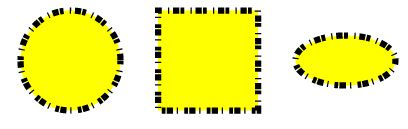
\includegraphics[width=0.7\linewidth]{obrazky/grupovanieElementov}
\caption{Príklad zoskupenia elementov a následná zmena atribútov}
\label{fig:grupovanieElementov}
\end{figure}

\subsection{Maskovanie - Paper.mask()}
Ekvivalentné správanie ako Paper.g až na to, že to je maska.  Vráti objekt mask element.  


\section{Gradient} 

Snap.svg  podporuje aplikovanie gradientov cez atribút fill s parametrom stringu gradientu. Cez metódu Paper.gradient(gradient) sa vytvorí gradientový element, ktorý sa dá nasledovne použiť ako hodnota pre atribút fill pre metódy Element.animate(), resp. Element.attr(). 
Gradientový string vyrezá nasledovne: $<$typ$>$($<$suradnice$>$)$<$farby$>$ .
\begin{itemize}
\item Typ môže byť buď lineárny alebo radiálny. Veľkosť písma určuje či ide o absolútne, alebo relatívne súradnice.
\item Súradnice špecifikujú lineárny gradient ako vektor x1, y1, x2, y2 alebo radiálny gradient ako cx, cy, r.Nepovinné sú fx, fy, ktoré špecifikujú ohniskový bod od centra kruhu. 
\item Farby je list pomlčkou oddelených hodnôt CSS farieb. Každá farba môže byť nasledovaná vlastným offsetovou hodnotou, oddelenou dvojbodkovým znakom. 
\end{itemize}

Lineárny grandient, vzťažný na horný ľavý roh do pravého dolného rohu. Farby prechádzajú z čiernej cez červenú do bielej.  
\begin{lstlisting}
var g = paper.gradient("l(0, 0, 1, 1)#000-#f00-#fff");
\end{lstlisting}

Lineárny gradient, absolútne z (0,0) do (100,100) z čiernej cez červenú na 25 percentách do bielej. 
\begin{lstlisting}
var g = paper.gradient("L(0, 0, 100, 100)#000-#f00:25-#fff");
\end{lstlisting}

Radiálny gradient, relatívny zo stredu elemetnu s polomerom polovice šírky, z čiernej do bielej. 
\begin{lstlisting}
var g = paper.gradient("r(0.5, 0.5, 0.5)#000-#fff");
\end{lstlisting}


Aplikovanie gradientu: 
\begin{lstlisting}
paper.circle.attr({fill: g});
\end{lstlisting}



\section{Práca s textom - Paper.text(x, y, text)}

Vykreslenie textu na plátne namiesto HTML markup s CSS štýlovaným umožňuje animovať a transformovať v rovnakým spôsobom ako iné tvary. Text vytvorení cez metódu text. Parametre metódy text sú súradnice x, y a text, ktorý sa vykreslí. Vlastnosti textu sa dajú zmeniť volaním metódy attr. V tabuľke sú atribúty, ktoré sa dajú zmeniť prostredníctvom metódy attr. 


\begin{table}[H]
	\begin{center}
		\begin{tabular}{|l|l|p{8cm}|}
			\hline \textbf{Snap atribút}  &\textbf{ CSS atribút}  & \textbf{Poznámka} \\ 
						\hline
			\hline font & font & napr. "30px Helvetica, sans-serif",\\ 
			\hline textAnchor & text-anchor & pozícia textu, napr. "middle" \\ 
			\hline fill & fill & výplň textu farbou, gradientom, vzorom \\ 
			\hline fontSize  & font-size  & veľkosť textu  \\ 
			\hline fontFamily & font-family & napr. "monospace" \\ 
			\hline fontStyle & font-style  & štýl písma, napr. kurzíva  \\ 
			\hline fontVariant  & font-variant  & napr. "small-caps"  \\ 
			\hline fontWeight & font-weight  &  hrúbka písma,  napr. normal, bold, bolder, lighter, 100-900\\ 
			\hline 
		\end{tabular} 
	\end{center}
\label{tab:text}
\caption{Atribúty na zmenu vlastností elementu text}
\end{table}

Príklad zmeny farby: 
\begin{lstlisting}[language = html]
var paper = Snap();
var text = paper.text(30, 100, "Namestovo");

text.attr({
	textAnchor: "middle", 	fill: "#00b", 	fontSize: '16px', 	fontFamily: "Veranda", 	fontStyle: "italic", 	fontVariant: "small-caps", 	fontWeight: 800, 
});
\end{lstlisting}

\section{Transformácie - Element.transform(...)}

Transformácia je realizovaná cez metódu Element.transform(), ktorá má v parametri transformačný string. Pri transformácii sa dá využiť klonovanie elementov cez metódu Element.clone(). Syntax transformačného stringu je vyjadrené z príkazov, ktoré sú v tabuľke \ref{tab:trasf}. 

\begin{table}[H]
	\begin{center}
		\begin{tabular}{|c|c|c|c|}
			\hline \textbf{Názov} & \textbf{Príkaz} & \textbf{Parameter} & \textbf{Príklad} \\ 
			\hline Posunutie & T, t & x, y & t50,100 \\ 
			\hline Rotácia& R, r & uhol, (bod rotacie x, y) & r45,0,0 \\ 
			\hline Škála & S, s & scale x, y, (scale bod x, y) & S 2,4.5,75,125 \\ 
			\hline 
		\end{tabular} 	
	\end{center}
	\label{tab:trasf}
	\caption{Syntax transformačného stringu pre Snap API}
\end{table}

Transformačný string využíva malé a veľké varianty príkazov. Variant s veľkými písmenami znamená to, že sa transformuje, bez ohľadu na predchádzajúcu transformáciu. Opačne to je pri variante s malými písmenami, ktoré berú na vedomie predošlú transformáciu.\cite[p.~52]{Dawber} 

V SVG SMIL sa vytvorí k elementu nový tag animateTransform, kde sa nastaví attributeName na transform, a typ a hodnoty sú uvedené v tabuľke \ref{tab:svgTrans}. 

\begin{table}[H]
	\begin{center}
		\begin{tabular}{|l|p{9cm}|}
			\hline \textbf{Transformation} & \textbf{Popis} \\ 
			\hline translate(x,y) & Posunie súradnicový systém na dané x, y.  \\ 
			\hline scale(xFactor, yFactor) & zmena mierky, \\ 
			\hline rotate(uhol) & Zrotuje súradnice o daný uhol.  \\ 
			\hline rotate(uhol, centerX, centerY) & Zrotuje súradnice o daný uhol, v daných bodoch.  \\ 
			\hline skewX(uhol) &  Skosenie pozdĺž osi X.  \\ 
			\hline skewY(uhol) &  Skosenie pozdĺž osi Y.  \\ 
			\hline 
		\end{tabular} 
		
	\end{center}
	\label{tab:svgTrans}
	\caption{Typy transformácií vo vnútri SVG tagu animateTransform }
\end{table}

\section{Animácie}

Snap.svg umožňuje animovať SVG grafické komponenty priamo manipulovaním jeho atribútov v JavaScripte. 

Element.animate(attr, ms, easing, callback). 
Parametre sú v tabuľke \ref{fig:animacie}
\begin{table}[H]
	\begin{center}
		\begin{tabular}{|c|p{10cm}|}
			\hline \textbf{Parameter} & \textbf{Popis} \\ 
			\hline attr &   Atribúty požadovaného elementu sú zadané v pároch - typ atribútu a jeho hodnota \\ 
			\hline duration &   Trvanie animácie v milisekundách \\ 
			\hline easing & zjemnenie animácie, mina objekt \\ 
			\hline callback & Funkcia, ktorá sa spustí po skončení animácie  \\ 
			\hline 
		\end{tabular} 
	\end{center}

	\caption{Parametre pre metódu animate}
		\label{fig:animacie}
\end{table}

\subsubsection{Animácia metód a jednoduchých atribútov animácie }

Jednoduché atribúty elementov, ktorých prechod sa zanimuje sú v časti o atribútoch elementov. Ako atribút sa dá použiť aj CSS3 atribút, ale musí byť v úvodzovkách, ak neexistuje v knižnici Snap.svg jeho ekvivalentný názov. 

\subsubsection{Animovanie path}

Pre animovanie zmeny tvaru jedného grafického komponentu na druhý sa využíva atribút path. Grafický element sa plynulo zanimuje, pretvaruje na tvar, ktorý je udaný. 

\subsection{Animácie transformácie}

Animovanie transformácie atribútu elementu využíva transformačný string.  Syntax: 
\begin{lstlisting}
	Element.animate({transform: [transformacny string]});
\end{lstlisting}


\section{Ďalšie metódy v knižnici Snap.svg}

\subsection*{Snap.load(url, callback, [scope])}
Načíta externý .svg súbor ako fragment. 
\subsection*{Element.append(...), Element.add(...), }
Slúži na pridanie, zobrazenie elementu na danom plátne. 
\subsection*{Element.stop()}
Zastaví všetky animácie pre súčastný element. Vracia súčastný element. 
\subsection*{Element.remove()}
Odstráni element z DOM. 
\subsection*{Element.removeData([key])}
Odstráni hodnotu asociovanú s elementom s daným kľúčom. Ak kľúč nie je zadaný, odstráni všetky dáta z elementu. 
\subsection*{Snap.select(...)}
Slúži na wrapovanie DOM elementu špecifikovaný CSS selektorom.  
\subsection*{Element.getBBox()}
Vráti bounding box opisovač pre daný element. Bounding box vyjadruje hranice elementu cez obdĺžnik. 

Vráti objekt s nasledujúcimi atribútmi: 
\begin{itemize}
	\item cx, cy - x, y stredu elementu,
	\item h, height - výška elementu,
	\item path - príkaz path pre daný box
	\item r0 - polomer kruhu, ktorý plne uzatvára box, 
	\item r1 - polomer najmenšieho kruhu, ktorý môže byť opísaný ku box,
	\item r2 - polomer najväčšieho kruhu, ktorý môže byť opísaný ku box, 
	\item vb - string -box ako viewbox príkaz
	\item w, width - šírka elemetnu 
	\item x2 - x súradnica pravej strany, 
	\item x - x súradnica ľavej strany, 
	\item y2 - y súradnica spodnej hrany, 
	\item y - y hornej hrany. 
\end{itemize}